\documentclass{article}

\usepackage[a4paper, total={6in, 8.5in}]{geometry}
%\usepackage[utf8]{inputenc}
%\usepackage[T1]{fontenc}    
%\usepackage{hyperref} 
%\usepackage{url}   
%\usepackage{booktabs}    
\usepackage{amssymb,amsfonts,amsmath,graphicx}      
%\usepackage{nicefrac}       
%\usepackage{microtype}    
%\usepackage{breqn}
%\usepackage[usenames, dvipsnames]{color}

\newcommand{\ind}[1]{1_{#1}} % Indicator function
\newcommand{\pr}{P} % Generic probability
\newcommand{\ex}{E} % Generic expectation
\newcommand{\var}{\textrm{Var}}
\newcommand{\cov}{\textrm{Cov}}
\newcommand{\sgn}{\textrm{sgn}}
\newcommand{\sign}{\textrm{sign}}
\newcommand{\kl}{\textrm{KL}} 
\newcommand{\abs}[1]{|{#1}|}



\renewcommand{\S}{\Sigma}
\renewcommand{\L}{\Lambda}
\renewcommand{\[}{\begin{equation}}
\renewcommand{\]}{\end{equation}}
\renewcommand{\b}{\backslash}
\newcommand{\g}{\,\vert\,}
\newcommand{\tr}{\mathrm{tr}}
\newcommand{\diag}{\mathrm{diag}}
\newcommand{\bea}{\begin{eqnarray}}
\newcommand{\eea}{\end{eqnarray}}
\newcommand{\hx}{\hat{x}}
\newcommand{\hxi}{\hat{\xi}}
\newcommand{\Var}{\mathrm{Var}}
\newcommand{\Cov}{\mathrm{Cov}}
\newcommand{\prop}{\propto}
\newcommand{\deq}{:=}

\newcommand{\EE}{\mathbb{E}}
\newcommand{\II}{\mathbb{I}}
\newcommand{\R}{\mathbb{R}}
\newcommand{\PP}{\mathbb{P}}

\newcommand{\La}{\mathcal{L}}

\newcommand{\n}{\mathcal{N}}

\newcommand{\bx}{\mathbf{x}}
\newcommand{\bX}{\mathbf{X}}
\newcommand{\by}{\mathbf{y}}
\newcommand{\bs}{\mathbf{s}}
\newcommand{\bn}{\mathbf{n}}
\newcommand{\br}{\mathbf{r}}
\newcommand{\bt}{\mathbf{t}}

\newcommand{\fig}[1]{Figure~\ref{fig:#1}}
\newcommand{\chap}[1]{Chapter~\ref{chap:#1}}
\newcommand{\mysec}[1]{Section~\ref{sec:#1}}
\newcommand{\app}[1]{Appendix~\ref{sec:#1}}
\newcommand{\eq}[1]{Eq.~(\ref{eq:#1})}
\newcommand{\eqs}[1]{Eqs.~(\ref{eq:#1})}
\newcommand{\eqss}[1]{(\ref{eq:#1})}
\newcommand{\thm}[1]{Theorem~\ref{thm:#1}}

\newcommand{\indep}{{\;\bot\!\!\!\!\!\!\bot\;}}
\newcommand{\eps}{\varepsilon}

\newcommand{\one}{1}
\newcommand{\Dir}{{\rm Dir}}
\newcommand{\Mult}{{\rm Mult}}
\newcommand{\Bin}{{\rm Bin}}
\newcommand{\Ga}{{\rm Ga}}
\newcommand{\IG}{{\rm IG}}
\newcommand{\InvGa}{{\rm IG}}
\newcommand{\Chisquare}{\Chi^2}
\newcommand{\St}{{\rm St}}
\newcommand{\Beta}{{\rm Beta}}
\newcommand{\iid}{i.i.d.}
\newcommand{\Eta}{{\cal N}}
\newcommand{\Ber}{{\rm Ber}}

\newcommand{\simiid}{\stackrel{\tiny\text{iid}}{\sim}}
\newcommand{\simind}{\stackrel{\tiny\text{ind}}{\sim}}

\DeclareMathOperator*{\BP}{BP}
\DeclareMathOperator*{\DP}{DP}
\DeclareMathOperator*{\GP}{GP}
\DeclareMathOperator*{\BeP}{BeP}

% Caligraphic alphabet
\newcommand{\calr}{\mathcal{R}} % only because \cr already taken
\newcommand{\ca}{\mathcal{A}} \newcommand{\cb}{\mathcal{B}} \newcommand{\cc}{\mathcal{C}} \newcommand{\cd}{\mathcal{D}} \newcommand{\ce}{\mathcal{E}} \newcommand{\cf}{\mathcal{F}} \newcommand{\cg}{\mathcal{G}} \newcommand{\ch}{\mathcal{H}} \newcommand{\ci}{\mathcal{I}} \newcommand{\cj}{\mathcal{J}} \newcommand{\ck}{\mathcal{K}} \newcommand{\cl}{\mathcal{L}} \newcommand{\cm}{\mathcal{M}} \newcommand{\cn}{\mathcal{N}} \newcommand{\co}{\mathcal{O}} \newcommand{\cp}{\mathcal{P}} \newcommand{\cq}{\mathcal{Q}} \newcommand{\cs}{\mathcal{S}} \newcommand{\ct}{\mathcal{T}} \newcommand{\cu}{\mathcal{U}} \newcommand{\cv}{\mathcal{V}} \newcommand{\cw}{\mathcal{W}} \newcommand{\cx}{\mathcal{X}} \newcommand{\cy}{\mathcal{Y}} \newcommand{\cz}{\mathcal{Z}}

% Convergence
\newcommand{\convd}{\stackrel{d}{\longrightarrow}} % convergence in distribution/law/measure
\newcommand{\convp}{\stackrel{P}{\longrightarrow}} % convergence in probability
\newcommand{\convas}{\stackrel{\textrm{a.s.}}{\longrightarrow}} % convergence almost surely
\newcommand{\convr}{\stackrel{r}{\longrightarrow}} % convergence in r^{th} mean

\newcommand{\eqd}{\stackrel{d}{=}} % equal in distribution/law/measure
\newcommand{\argmax}{\mathop{\mathrm{argmax}}}
\newcommand{\argmin}{\mathop{\mathrm{argmin}}}
\newcommand{\conv}{\textrm{conv}} % for denoting the convex hull


\makeatletter
\providecommand*{\diff}%
	{\@ifnextchar^{\DIfF}{\DIfF^{}}}
\def\DIfF^#1{%
	\mathop{\mathrm{\mathstrut d}}%
		\nolimits^{#1}\gobblespace}
\def\gobblespace{%
	\futurelet\diffarg\opspace}
\def\opspace{%
	\let\DiffSpace\!%
	\ifx\diffarg(%
		\let\DiffSpace\relax
	\else
		\ifx\diffarg[%
			\let\DiffSpace\relax
	\else
		\ifx\diffarg\{%
			\let\DiffSpace\relax
		\fi\fi\fi\DiffSpace}


\providecommand*{\deriv}[3][]{\frac{\diff^{#1}#2}{\diff #3^{#1}}}
\providecommand*{\pderiv}[3][]{\frac{\partial^{#1}#2}{\partial #3^{#1}}}
		
\newcommand{\threequals}{\equiv}

\DeclareMathOperator*{\argminU}{arg\,min}
\DeclareMathOperator*{\argmaxU}{arg\,max}


\begin{document}


\section{Model}
\label{model}


\subsection{Basic Constituents}

\noindent Ideal Point Model (IPM)
\begin{itemize}
\item For each document $d$
\begin{enumerate}
\item Choose a discrimination $a_d \sim \cn(\eta_{a},\sigma^2_d)$
\item Choose a difficulty $b_d \sim \cn(\eta_{b},\sigma^2_d)$
\end{enumerate}
\item For each representative $u$
\begin{enumerate}
\item Choose a position $x_u\mid \nu \sim \cn(\nu,\sigma^2_x)$
\end{enumerate}
\item Draw representative $u$'s vote on document $d$ as $V_{ud} \mid x_u, a_d, b_d \sim \text{Bern}(\sigma(a_d\cdot(x_u-b_d)))$%, for $u\in\{1,\dots, U\}, d\in\{1,\dots,D\}$
\end{itemize}


\noindent Stochastic Block Model (SBM)
\begin{itemize}
\item Choose the community proportions $\pi \sim \text{Dir}(\gamma)$, where $\pi\in \R^K$ with $K$ latent communities
\item For each representative $u$
\begin{enumerate}
\item Choose a community membership assignment $M_u\simiid \text{Cat}(\pi)$
\end{enumerate}
\item For each pair of communities $k< l\in\{1,\dots, K\}$, draw coexpression rate $P_{kl} \simiid \text{Gamma}(\lambda_0,\lambda_1)$%, for $k,l\in \{1,\dots, C\}$
\item For each pair of representatives $u<v$, %\in\{1,\dots, U\}
 draw $R_{uv} \mid P, M_u=k, M_v=l\sim \text{Poisson}(P_{kl})$
\end{itemize}


\iffalse
\noindent Latent Dirichlet Allocation (LDA) 
\begin{itemize}
\item Draw a topic $\varphi_k \simiid \text{Dir}(\beta), \varphi_k\in \R^V$ as a distribution over words, for each $k\in\{1,\dots,K\}$ 
\item For each document, draw the topic proportions $\theta_d \simiid \text{Dir}(\alpha)$, where $\theta_d\in \R^K$ %, for $d\in\{1,\dots,D\}$
\item For each document $d\in\{1,\dots,D\}$ and each word $n\in\{1,\dots,N_d\}$ in the document
\begin{enumerate}
\item Choose a topic $z_{dn}\mid \theta_d \simind \text{Mult}(\theta_d)$ %, for $d\in\{1,\dots,D\}$, $n\in\{1,\dots,N_d\}$
\item Choose a word $W_{dn}\mid z_{dn}=k, \varphi_k\simind \text{Mult}(\varphi_k)$ %, for $d\in\{1,\dots,D\}$, $n\in\{1,\dots,N_d\}$
\end{enumerate}
\end{itemize}
\fi




\subsection{LC-IPM}

The ideal point model (IPM) is useful to us as a baseline model for the roll call voting data $(V_{ud})$ for a couple of reasons. For one, using it alone we can attempt to predict missing votes, a problem of interest in political science. Another problem of more qualitative interest is analyzing and interpreting the factors $a_d, b_d$ specific to a document and those $x_u$ specific to the representative. All are assumed to reside in some latent space $\R^S$ and so depending on how we set up the model, we might be able to interpret quantities like $x_u$ as $u$'s {\sl political stance} or {\sl ideological position} or $x_u - b_d$ as representative $u$'s propensity for the bill/document $d$. There are a number of problems we cannot address in IPM. A major problem is predicting on heldout documents (the `cold start'), which is a potentially useful performance measure. Similarly if we have relatively junior representatives, they may not have had enough votes for the inferred $x_u$ to represent something (1) meaningful / interpretable or (2) reliable. We want to incorporate more information to inform the choices of $a_d, b_d$ and $x_u$. We focus on the latter, with an interest in being able to better interpret the ideal points of the representatives. We use the stochastic block model to model the assumption that representatives `vote in groups' in the sense that they belong to various communities which tend to have the similar positions.
~\\

\newpage


\noindent Latent Community-Ideal Point Model%Ideal Point Allocator (IPA)
\begin{itemize}
\item Run the generative processes for SBM as described above. Then, % and LDA
\item For each document $d$ (as before)
\begin{enumerate}
%\item Calculate the empirical topic proportions $\overline z_d  = \frac{1}{N_d}\sum_{i=1}^{N_d}z_d$ (a $K\times 1$ vector)
%\item Generate $S\times K$ matrices $\eta_a, \eta_b$ with iid normal entries 
\item Choose a discrimination $a_d \sim \cn(\eta_{a},\sigma^2_d)$ %$a_d \sim \cn(\eta_{a}'\overline z_d,\sigma^2_d)$
\item Choose a difficulty $b_d \sim \cn(\eta_{b},\sigma^2_d)$
\end{enumerate}
\item For each representative $u$
\begin{enumerate}
\item Generate the community means $\nu_k\sim \cn(\varpi, \sigma^2_x)$
\item Choose a position $x_u\mid M_u = k, \nu \sim \cn(\nu_k,\sigma^2_x)$
\end{enumerate}
\item Draw representative $u$'s vote on document $d$ as $V_{ud} \mid x_u, a_d, b_d \sim \text{Bern}(\sigma(a_d\cdot(x_u-b_d)))$
\end{itemize}



\begin{figure}[h]
  \centering
  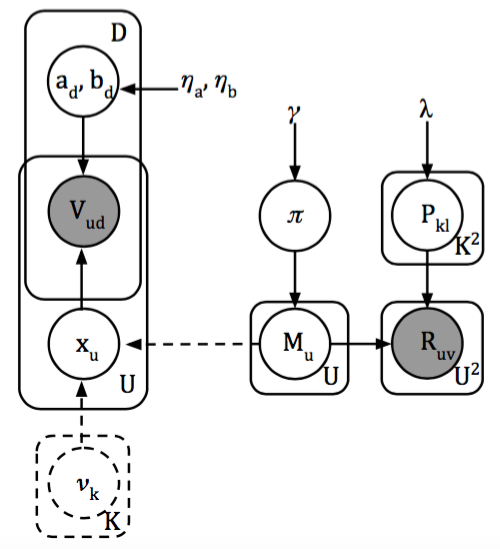
\includegraphics[scale=.4]{lcipm2}
  \caption{LC-IPM graphical model}
\end{figure}

\newpage

\section{Variational Inference}
\label{vi}

\subsection{For SBM.} After observing the symmetric matrix $R = (R_{uv})$, where $R_{uv}$ is the number of caucuses that representatives $u$ and $v$ have in common, we see to find a distribution $q$ over the latent community assignments $M = (M_u)$, the community coexpression rates $P = (P_{kl})$, and the community proportions $\pi = (\pi_k)$ which is close in relative entropy to the true posterior and lies in the factorized family $q(M)q(P)q(\pi)$. Each factor has free parameters described below and denoted with $\widehat{\text{hats}}$. The approximation $q$ is equivalently scored by the ELBO objective $\cl$, which we break down as:%arrange into component terms:
\begin{equation}
\begin{split}
\cl(q)
&= \EE_q\left[\log\frac{p(R,M,P,\pi)}{q(M,P,\pi)}\right]  \\
&= \underbrace{\EE_q\left[\log p(R\mid M,P)+ \log\frac{p(P)}{q(P)}\right]}_{\cl_{\text{data}}}
+ \underbrace{\EE_q\left[-\log q(M)\right]}_{\cl_{\text{ent}}}
+ \underbrace{\EE_q\left[\log p(M\mid \pi)\right]}_{\cl_{\text{local}}}
+ \underbrace{\EE_q\left[\log\frac{p(\pi)}{q(\pi)}\right]}_{\cl_{\text{global}}}
\end{split}
\end{equation}

\noindent{\bf Variational Factors.} To each $u$ we associate variational parameters $\widehat r_u = \left(\widehat r_{uk}\right)_{k=1}^C$, so
\begin{align}
q(M) = \prod_{u=1}^U q(M_u\mid \widehat r_u) 
= \prod_{u=1}^U \prod_{k=1}^C \widehat r_{uk}^{\delta_k(M_u)}.
\end{align}
We define $q(\pi) \triangleq \text{Dir}(\widehat \gamma_1, \dots, \widehat \gamma_C)$ and $q(P) = \prod_{kl}q(P_{kl}\mid \widehat \lambda_{kl})$ where $q(P_{kl}\mid \widehat \lambda_{kl})\triangleq \text{Gamma}(\widehat \lambda_{0kl},\widehat \lambda_{1kl})$. \\

\noindent{\bf Computing the ELBO.} Now we can write out the component terms of the ELBO more explicitly:
\begin{equation}
%\hspace{-12em}
\begin{split}
\cl_{\text{data}}
&= \EE_q\left[\log p(R\mid M,P)+ \log\frac{p(P)}{q(P)}\right]
= \sum_{kl}\EE_q\left[\sum_{u,v}\delta_{k}(M_u)\delta_l(M_v)\log p(R_{uv}\mid P_{kl})+ \log\frac{p(P_{kl})}{q(P_{kl})}\right] \\
%&= \sum_{kl}\EE_q\left[\sum_{u,v}\delta_{k}(M_u)\delta_l(M_v)\log \frac{e^{-P_{kl}}}{R_{uv}!}P_{kl}^{R_{uv}}+ \lambda_{0}\log\lambda_1-\widehat\lambda_{0kl}\log\widehat\lambda_{1kl} - \log\frac{\Gamma(\lambda_0)}{\Gamma(\widehat\lambda_{0kl})} + (\lambda_0-\widehat\lambda_{0kl})\log P_{kl} - (\lambda_1-\widehat\lambda_{1kl})P_{kl}\right] \\ %%
&= -\sum_{u,v}\log R_{uv}! + \sum_{k,l} \left(\lambda_{0}\log\lambda_1-\widehat\lambda_{0kl}\log\widehat\lambda_{1kl} - \log\frac{\Gamma(\lambda_0)}{\Gamma(\widehat\lambda_{0kl})}\right) + \sum_{k,l} \cl_{kl}(R)
~\\
\cl_{\text{ent}}
&= \EE_q\left[-\log q(M)\right]
= -\sum_{u,k}\EE_q\left[\delta_{k}(M_u)\log \widehat r_{uk}\right]
= -\sum_{u,k}\widehat r_{uk}\log \widehat r_{uk}
~\\
\cl_{\text{local}}
&= \EE_q\left[\log p(M\mid \pi)\right]
= \sum_{u,k}\EE_q\left[\delta_{k}(M_u)\log \pi_k\right]
= \sum_{k}N_k\EE_q\left[\log \pi_k\right]
~\\
\cl_{\text{global}}
&= \EE_q\left[\log\frac{p(\pi)}{q(\pi)}\right]
= \log \Gamma(C\gamma) - C\log\Gamma(\gamma) -\log \Gamma\left(\sum_k\widehat\gamma_k\right) + \sum_k\left\{\log\Gamma(\widehat\gamma_k)+ (\gamma-\widehat\gamma_k)\EE_q\left[\log \pi_k\right]\right\}
\end{split}
\end{equation}
where $N_k = \sum_{u}\widehat r_{uk}$, $S_{uk} = \sum_{v}\widehat r_{vk}R_{uv}$, $N_{kl} = \sum_{uv}\widehat r_{uk}\widehat r_{vl}$, $S_{kl} = \sum_{uv}\widehat r_{uk}\widehat r_{vl} R_{uv}$, and 
$$
\cl_{kl}(R) 
= (S_{kl} + \lambda_{0} - \widehat\lambda_{0kl}) \EE_q[\log P_{kl}]
   -(N_{kl} + \lambda_{1} - \widehat\lambda_{1kl}) \EE_q[P_{kl}], 
$$
and the posterior expectations can also be computed explicitly as 
$$
\EE_q[P_{kl}] =  \frac{\widehat\lambda_{0kl}}{\widehat\lambda_{1kl}}, ~
\EE_q[\log P_{kl}] = \psi(\widehat\lambda_{0kl}) - \log \widehat\lambda_{1kl}, ~
\EE_q\left[\log \pi_k\right] = \psi\left(\widehat\gamma_k\right) - \psi\left(\sum_l\widehat\gamma_l\right)
$$

\newpage

\noindent{\bf CAVI Updates.} The simplest approach to variational inference maximizes the ELBO $\cl$ via coordinate-ascent, i.e. choosing the best value of a variational parameter with all others fixed. Iteratively applying these updates, the variational approximation $q$ improves at every step toward some local optimum. Conditional conjugacy yields closed form updates for the global variational parameters. 

\begin{itemize}
\item {\bf Global Update to $q(\pi)$.} We have $\widehat \gamma_{k} = \gamma + N_k$.
\item {\bf Global Update to $q(P)$.} We have $\widehat \lambda_{0kl} = \lambda_0 + S_{kl}$ and $\widehat \lambda_{1kl} = \lambda_1 + N_{kl}$.
\item {\bf Local Update to $q(M)$.} Differentiating the ELBO with respect to $\widehat r_{uk}$,

\iffalse
First note 
%$$ \pderiv{\cl_{kl}}{\widehat r_{uk}} = \left(\sum_{v}(1+\delta_u^v\delta_k^l)\widehat r_{vl}R_{uv}\right) \EE_q[\log P_{kl}] -N_l \EE_q[P_{kl}]$$
$$ 
\pderiv{\cl_{kl}}{\widehat r_{uk}} 
= \left\{
                \begin{array}{ll}
%2\sum_{v}\widehat r_{vk} R_{uv}\EE_q[\log P_{kk}]
%2S_{uk}\EE_q[\log P_{kk}] - 2N_k \EE_q[P_{kk}],
(S_{uk}+\hat r_{uk}R_{uu})\EE_q[\log P_{kk}] - 2N_k \EE_q[P_{kk}],
  ~~~~ k=l \\
%\sum_{v}\widehat r_{vl} \left(R_{uv} \EE_q[\log P_{kl}] - \EE_q[P_{kl}]\right)
S_{ul} \EE_q[\log P_{kl}] - N_l\EE_q[P_{kl}]
  ~~~~ k\neq l
                \end{array}
              \right.
$$
We want to update $\widehat r_{uk}$ subject to the constraint that $\sum_k \widehat r_{uk} = 1$, so augment $\cl$ with Lagrange multipliers $\widetilde\cl = \cl + \sum_u\kappa_u\left(\sum_k \widehat r_{uk} - 1\right)$.

\begin{align*}
0 
&= \pderiv{\cl}{\widehat r_{uk}}
= -\log \widehat r_{uk} - 1 + \EE_q\left[\log \pi_k\right] + \pderiv{\cl_{kk}}{\widehat r_{uk}} + \sum_{l\neq k}\pderiv{\cl_{kl}}{\widehat r_{uk}} + \pderiv{\cl_{lk}}{\widehat r_{uk}} \\
&= -\log \widehat r_{uk} - 1 + \EE_q\left[\log \pi_k\right] + \sum_{l} S_{ul}\left(\EE_q[\log P_{kl}] + \EE_q[\log P_{lk}]\right) - N_l\left(\EE_q[P_{kl}] + \EE_q[P_{lk}]\right)\\
\end{align*}
\fi

$$
0 = \pderiv{\cl}{\widehat r_{uk}}= -\log \widehat r_{uk} -1 + \EE_q[\log \pi_k]
+ \sum_{v\neq u} \sum_l \widehat r_{vl}\left(R_{uv}\EE_q[\log P_{kl}] - \EE_q[P_{kl}]\right).
$$
Thus, we take 
$$
\widehat r_{uk} \propto_k \exp\left(\EE_q[\log \pi_k]
+ \sum_{v\neq u} \sum_l \widehat r_{vl}\left(R_{uv}\EE_q[\log P_{kl}] - \EE_q[P_{kl}]\right)\right)
$$


\end{itemize}


\newpage


\subsection{For IPM}
We observe the votes matrix $V = (V_{ud})$ where $V_{ud}$ is the vote of congressperson $u$ on bill $d$. We have the ideal point for congressperson $u$, $x_u \in \R^s$, and the discrimination and difficulty for bill $d$, $a_d,b_d \in \R^s$. The variational distribution is the fully factorized family $\prod_{u=1}^U \prod_{d=1}^D q(x_u)q(a_D)q(b_d)$ where $q(x_u) \triangleq \text{Normal}(\hat{\tau}_u, \hat{\sigma}^2_\tau I_S)$, $q(x_u) \triangleq \text{Normal}(\hat{\kappa}_{au}, \hat{\sigma}^2_{\kappa_a} I_S)$, and $q(x_u) \triangleq \text{Normal}(\hat{\kappa}_{bu}, \hat{\sigma}^2_{\kappa_b} I_S)$
\vskip 10pt
\noindent{\textbf{Computing the ELBO.}} 
We can write the ELBO as 
\begin{align*}
\cl(q) & = \EE_q\left[-\sum_{u=1}^U\log q(x_u) - \sum_{d=1}^D \log q(a_d) - \sum_{d=1}^D \log q(b_d)\right] + \EE_q\left[\sum_{u=1}^U \log p(X_{u}) +\sum_{d=1}^D \log p(a_d) + \sum_{d=1}^D \log p(b_d)\right]\\
& \;\;\;\; + \EE_q[\log p(V|x,a,b)]\\
& = H(q) +  \EE_q\left[\sum_{u=1}^U \log p(X_{u}) +\sum_{d=1}^D \log p(a_d) + \sum_{d=1}^D \log p(b_d)\right] + \EE_q[\log p(V|x,a,b)]\\
\end{align*}

We can break this up into 
\begin{align*}
H(q) & = U\frac{S}{2} \log 2\pi e\hat{\sigma}^2_\tau + D\frac{S}{2}\log 2\pi e\hat{\sigma}^2_{\kappa_a} + D\frac{S}{2}\log 2\pi e\hat{\sigma}^2_{\kappa_b}\\
\EE_q\left[\sum_{u=1}^U \log p(X_{u})\right] & = \sum_{u=1}^U \EE_q\left[-\frac{S}{2} \log 2\pi \sigma^2_x - \frac{1}{2\sigma^2_x} \|x_u - \nu\|_2^2\right]\\
& = -U\frac{S}{2} - \frac{1}{2\sigma^2_x} \sum_{u=1}^U \hat{\sigma}^2_\tau S + \|\hat{\tau}_u - \nu\|^2_2\\
\EE_q\left[\sum_{d=1}^D \log p(a_d)\right] & = \sum_{d=1}^D \EE_q\left[-\frac{S}{2} \log 2\pi \sigma^2_a - \frac{1}{2\sigma^2_a} \|a_d - \eta_a\|_2^2\right]\\
& = -D\frac{S}{2} - \frac{1}{2\sigma^2_a} \sum_{d=1}^D \hat{\sigma}^2_{\kappa_a} S + \|\hat{\kappa}_{ad} - \eta_a\|^2_2\\
\EE_q\left[\sum_{d=1}^D \log p(b_d)\right] & = \sum_{d=1}^D \EE_q\left[-\frac{S}{2} \log 2\pi \sigma^2_b - \frac{1}{2\sigma^2_b} \|b_d - \eta_b\|_2^2\right]\\
& = -D\frac{S}{2} - \frac{1}{2\sigma^2_b} \sum_{d=1}^D \hat{\sigma}^2_{\kappa_b} S + \|\hat{\kappa}_{bd} - \eta_b\|^2_2\\
\end{align*}
We can deal with the last expectation by using the 2nd order delta method (Braun McAullife 2008) which is the approximation
\begin{align*}
\EE[f(V)] \approx f(\EE[V]) + \frac{1}{2} \text{trace}\left(\nabla^2 \EE[V] \Cov(V)\right)
\end{align*}
Letting $u(i),d(i)$ be the users and documents for data point $i$, and applying this gives the approximation to the ELBO contribution from the likelihood
\begin{align*}
\EE_q[\log p(V|x,a,b)] & = \sum_{i=1}^n \EE_q[V_i(a_{d(i)} \cdot (X_{u(i)} - b_{d(i)}))] + \EE_q[\log (1-\sigma(a_{d(i)} \cdot (X_{u(i)} - b_{d(i)})))]\\
& \approx \sum_{i=1}^nV_i (\hat{\kappa}_{ad(i)} \cdot (\hat{\tau}_{u(i)} - \hat{\kappa}_{bd(i)}) - \log (1 + \exp(\hat{\kappa}_{ad(i)} \cdot (\hat{\tau}_{u(i)} - \hat{\kappa}_{bd(i)})\\
& \;\;\;\; - \frac{1}{2} \sigma''(\hat{\kappa_{ad(i)}} \cdot (\hat{\tau}_{u(i)} - \hat{\kappa}_{bd(i)})(\hat{\sigma}^2_{\kappa_a} \|\hat{\tau}_{u(i)} - \hat{\kappa}_{bd(i)}\|_2^2 + (\hat{\sigma}^2_{\tau} + \hat{\sigma}^2_{\kappa_b})\|\hat{\kappa}_{ad(i)}\|^2)
\end{align*}
Where $\sigma(\cdot)$ is the sigmoid function.
\vskip 10pt
\noindent{\textbf{CAVI Updates.}} There are no closed form updates for $\hat{\tau}_u$, $\hat{\kappa}_{ad}$, and $\hat{\kappa}_{bd}$, so we have to maximize the ELBO with respect to these parameters numerically. Let $V(u)$ be the set of votes for user $u$, and similarly let $V(d)$ be the set of votes on bill $d$. Also let $\rho_{ud} = \sigma(\hat{\kappa_{ad(i)}} \cdot (\hat{\tau}_{u(i)} - \hat{\kappa}_{bd(i)})$. The gradients are
\begin{align*}
\nabla_{\hat{\tau}_u} \cl & = \frac{1}{\sigma^2_x}(\hat{\tau}_u - \nu) + \sum_{i \in V(u)}(V_i - \rho_{ud(i)})\hat{\kappa}_{ad(i)}\\
& \;\;\;\; - \frac{1}{2} \sigma''(\hat{\kappa}_{ad(i)} \cdot (\hat{\tau}_{u} - \hat{\kappa}_{bd(i)})(\hat{\sigma}^2_{\kappa_a} \|\hat{\tau}_{u} - \hat{\kappa}_{bd(i)}\|_2^2 + (\hat{\sigma}^2_{\tau} + \hat{\sigma}^2_{\kappa_b})\|\hat{\kappa}_{ad(i)}\|^2)\hat{\kappa}_{ad(i)}\\
& \;\;\;\; - \sigma'(\hat{\kappa}_{ad(i)} \cdot (\hat{\tau}_{u} - \hat{\kappa}_{bd(i)}))\hat{\sigma}^2_{ka}(\hat{\tau}_u - \hat{\kappa}_{bd(i)})\\
\nabla_{\hat{\kappa}_{ad}} \cl & = \frac{1}{\sigma^2_a}(\hat{\kappa}_{ad} - \eta_a) + \sum_{i \in V(d)}(V_i - \rho_{u(i)d})(\hat{\tau}_{u(i)} - \hat{\kappa}_{bd})\\
& \;\;\;\; - \frac{1}{2} \sigma''(\hat{\kappa}_{ad} \cdot (\hat{\tau}_{u(i)} - \hat{\kappa}_{bd})(\hat{\sigma}^2_{\kappa_a} \|\hat{\tau}_{u(i)} - \hat{\kappa}_{bd}\|_2^2 + (\hat{\sigma}^2_{\tau} + \hat{\sigma}^2_{\kappa_b})\|\hat{\kappa}_{ad}\|^2)(\hat{\tau}_{u(i)} - \hat{\kappa}_{bd})\\
& \;\;\;\; - \sigma'(\hat{\kappa}_{ad} \cdot (\hat{\tau}_{u(i)} - \hat{\kappa}_{bd})(\hat{\sigma}^2_{\tau} + \hat{\sigma}^2_{\kappa_b})\hat{\kappa}_{ad}\\
\nabla_{\hat{\kappa}_{bd}} \cl & = \frac{1}{\sigma^2_b}(\hat{\kappa}_{bd} - \eta_b) - \sum_{i \in V(d)}(V_i - \rho_{u(i)d})\hat{\kappa}_{ad}\\
& \;\;\;\; + \frac{1}{2} \sigma''(\hat{\kappa}_{ad} \cdot (\hat{\tau}_{u(i)} - \hat{\kappa}_{bd})(\hat{\sigma}^2_{\kappa_a} \|\hat{\tau}_{u(i)} - \hat{\kappa}_{bd}\|_2^2 + (\hat{\sigma}^2_{\tau} + \hat{\sigma}^2_{\kappa_b})\|\hat{\kappa}_{ad}\|^2)\hat{\kappa}_{ad}\\
& \;\;\;\; + \sigma'(\hat{\kappa}_{ad} \cdot (\hat{\tau}_{u(i)} - \hat{\kappa}_{bd})\hat{\sigma}^2_{ka}(\hat{\tau}_{u(i)} - \hat{\kappa}_{bd})
\end{align*}
For each parameter we solve this optimization problem using L-BFGS. Finally, there are closed form updates for the variational variance parameters by taking the derivative and setting to zero
\begin{align*}
\hat{\sigma}^2_\tau & = \frac{US}{\frac{US}{\sigma^2_x} + \sum_{i=1}^n \sigma'(\hat{\kappa_{ad(i)}} \cdot (\hat{\tau}_{u(i)} - \hat{\kappa}_{bd(i)}))(S\hat{\sigma^2}_{\kappa_a} + \|\hat{\kappa}_{ad(i)}\|_2^2)}\\
\hat{\sigma}^2_{\kappa_a} & = \frac{DS}{\frac{DS}{\sigma^2_a} + \sum_{i=1}^n \sigma'(\hat{\kappa_{ad(i)}} \cdot (\hat{\tau}_{u(i)} - \hat{\kappa}_{bd(i)}))(S(\hat{\sigma^2}_{\tau} + \hat{\sigma}^2_{\kappa_b}) + \|\hat{\tau}_{u(i)} - \hat{\kappa}_{bd(i)}\|_2^2)}\\
\hat{\sigma}^2_\tau & = \frac{DS}{\frac{DS}{\sigma^2_b} + \sum_{i=1}^n \sigma'(\hat{\kappa_{ad(i)}} \cdot (\hat{\tau}_{u(i)} - \hat{\kappa}_{bd(i)}))(S\hat{\sigma^2}_{\kappa_a} + \|\hat{\kappa}_{ad(i)}\|_2^2)}
\end{align*}







\newpage


\subsection{For LC-IPM}

The factorization for $q$ is the same, with one more factor $q(\nu) = \prod_kq(\nu_k)$ where $q(\nu_k)\triangleq \cn(\widehat\mu_k,\widehat\sigma^2_\mu)$. Due to the factorization in the LC-IPM generative model, the only contribution to the ELBO from IPM which changes is that corresponding to $(x_u)$. This becomes%; similarly, from SBM, corresponding to $(M_u)$. The former is
\begin{align*}
\cl_x 
&= \EE_q\left[\log \frac{p(x|\nu, M)}{q(x)}\right]
= \EE_q\left[\log \prod_{uk}\phi(x_u|\nu_k)^{\delta_k(M_u)}\right] + H(q) \\
&= \sum_{uk}\widehat r_{uk}\EE_q\left[\log \phi(x_u|\nu_k)\right] + H(q) 
\end{align*}
%forgetting constant terms, 
%\begin{align*}
%\cl_x 
%&= \sum_{uk}\widehat r_{uk}\left(-\frac{1}{2\sigma^2_x}\left(S(\widehat\sigma^2_\tau + \widehat\sigma^2_\mu) - \|\widehat\tau_u - \widehat\mu_k\|^2\right)\right)
%\end{align*}
In particular, the gradient of the ELBO w.r.t. the responsibility $\widehat r_{uk}$ is
\begin{align*}
0 
&= \pderiv{\cl_\text{SBM}}{\widehat r_{uk}} + \pderiv{\cl_x}{\widehat r_{uk}} \\
&= -\log \widehat r_{uk} - 1 + \EE_q\left[\log \pi_k\right] + \sum_{l} S_{ul}\left(\EE_q[\log P_{kl}] + \EE_q[\log P_{lk}]\right) - N_l\left(\EE_q[P_{kl}] + \EE_q[P_{lk}]\right)\\
&~~~+ \left(-\frac{1}{2\sigma^2_x}\left(S(\widehat\sigma^2_\tau + \widehat\sigma^2_\mu) - \|\widehat\tau_u - \widehat\mu_k\|^2\right)\right) + \EE_q\left[\log \phi(x_u|\nu_k)\right]
\end{align*}
so the update is
$$
\widehat r_{uk} \propto_k \exp\left(\EE_q[\log \pi_k]
+ \sum_{v\neq u} \sum_l \widehat r_{vl}\left(R_{uv}\EE_q[\log P_{kl}] - \EE_q[P_{kl}]\right)
+ \EE_q\left[\log \phi(x_u|\nu_k)\right]\right). 
$$
To determine the updates for the variational mean $\widehat \mu_k$ corresponding to $\nu_k$, we need the ELBO term
$$
\cl_\nu 
= \EE_q\left[\log \frac{p(\nu)}{q(\nu)}\right]
= \sum_k\EE_q\left[\log p(\nu_k)\right] + KH(q(\nu_1))
= -\frac{1}{2\sigma_\nu^2}\sum_k\|\widehat\mu_k-\varpi\|^2 + \frac{KS}{2}\log\left(2\pi e\widehat\sigma^2_\mu\right) + \text{const.}
$$
Setting the gradient of the ELBO w.r.t. $\widehat\mu_k$ equal to zero, we obtain
$$
0
= \pderiv{(\cl_\nu + \cl_x)}{\widehat\mu_k}
= \frac{1}{\sigma_x^2}\sum_u\widehat r_{uk}(\widehat\tau_u -\widehat\mu_k)  - \frac{1}{\sigma_\nu^2}(\widehat \mu_k - \varpi)
= \frac{1}{\sigma_x^2}\sum_u\widehat r_{uk}\widehat\tau_u -\left(\frac{N_k}{\sigma_x^2}+\frac{1}{\sigma_\nu^2}\right)\widehat\mu_k + \frac{1}{\sigma_\nu^2}\varpi
$$
and thus
$$
\widehat\mu_k= \left(\frac{\sum_u\widehat r_{uk}\widehat\tau_u}{\sigma_x^2} + \frac{\varpi}{\sigma_\nu^2}\right)\widehat\sigma^2_{\hat\mu_k}; \text{ where }
\widehat\sigma^2_{\hat\mu_k} = \left(\frac{N_k}{\sigma_x^2}+\frac{1}{\sigma_\nu^2}\right)^{-1}.
%\widehat\sigma_\mu^2 = \left(\frac{U}{K\sigma_x^2}+\frac{1}{\sigma_\nu^2}\right)^{-1}
$$

\newpage

\subsection{For LDA}
%\begin{align*}
%\end{align*}
For a particular document $d$, the posterior distribution for its topic distribution $\theta_d$ and the latent topics $\{z_{dn}\}_{n=1}^{N_d}$ for the $N_d$ words is given by
\begin{align*}
p(\theta_d, \{z_{dn}\}_{n=1}^{N_d} | \{w_{dn}\}_{n=1}^{N_d}, \alpha, \beta, a_d, b_d) 
&=\frac{ p(\theta_d | \alpha) \Big( \prod_{n=1}^{N_d} p(z_{dn} | \theta_d) p(w_{dn} | z_{dn}, \beta) \Big) p(a_d, b_d | \{z_{dn}\}_{n=1}^{N_d} , \eta, \sigma^2)}{\int  p(\theta_d | \alpha) \sum_{z_{\cdot d}}\Big( \prod_{n=1}^{N_d} p(z_{dn} | \theta_d) p(w_{dn} | z_{dn}, \beta) \Big) p(a_d, b_d | \{z_{dn}\}_{n=1}^{N_d} , \eta, \sigma^2) \; d\theta_d}
\end{align*}
In particular, the normalizer gives us the likelihood of the observed words $\{w_{dn}\}_{n=1}^{N_d}$ and the response $a_d$ and $b_d$. This is computationally intractable, so we apply a variational method in which we assume a fully factorized posterior distribution for $\theta_d$ and $z_{dn}$ of the form 
\begin{align*}
q(\theta_d, \{z_{dn}\}_{n=1}^{N_d} | \gamma, \{\phi_n\}_{n=1}^{N_d}) = q(\theta_d| \gamma) \prod_{n=1}^N q(z_{dn} | \phi_n)
\end{align*}
where $\phi_n$ is a vector on the symplex that gives the multinoulli probabilities of $z_{dn}$, and $\gamma$ is the $K$ dimensional Dirichlet parameter for $\theta_d$. With respect to these two variational parameters, we seek to maximize the evidence lower bound (ELBO) given by
\begin{align*}
\mathcal L (\gamma, \phi; \alpha, \beta, \eta, \sigma)  = E_q[\log p(\theta_d | \alpha) ] + &\sum_{n=1}^{N_d} E_q [\log p(z_{dn} | \theta)] +\sum_{n=1}^{N_d}  E_q[\log p(w_{dn}|z_{dn}, \beta)]+ ...\\ 
&+E[\log p(a_d, b_d  | \{z_{dn}\}_{n=1}^{N_d} , \eta, \sigma^2) ]
- E_q[\log q(\theta_d |\gamma) ] - \sum_{i=1}^{N_d}E([\log q(z_{dn} | \phi_n) ] )
\end{align*}
The updates for $\phi_j$ ($j\in \{1, ..., N_d\}$) and $\gamma$ were derived in (Blei \& McAuliffe, 2008) and given by
\begin{align*}
\phi^{new}_j \propto \exp\bigg\{ E[\log \theta_d | \gamma] + E[\log p(w_{dn} | \beta)] + \Big(\frac{y}{N_d\sigma^2} \Big) \eta - \frac{[2(\eta^T\phi_{-j})\eta + (\eta \circ \eta)]}{2N_d^2\sigma^2}\bigg\}
\end{align*}
where $\phi_{-j} := \sum_{n\not=j} \phi_n$; and $E(\log \theta_i | \gamma] = \Psi(\gamma_i) - \Psi(\sum \gamma_j)$, where $\Psi$ is the digamma function. Now the updates for $\gamma$ is: 
\begin{align*}
\gamma^{new} &\rightarrow \alpha + \sum_{n=1}^{N_d} \phi_n 
\end{align*}
These give the updates for a single document response pair. Having updated $\gamma_d$ and $\phi_d$ for each document, the updates for $\beta$ are given by examing the entire corpus (Blei et al, 2003): 
\begin{align*}
\beta^{new}_{k,w} &\propto \sum_{d=1}^D \sum_{n=1}^{N_d} 1\{(w_{dn} = w)\} \phi^k_{d,n}
\end{align*}


\newpage 

\section{Model}
%We introduce models for both roll call votes and caucus memberships. 

\subsection{Ideal point model}

\subsection{Stochastic Block Models} 

\end{document}

